\documentclass[12pt, a4paper, oneside]{article}
\usepackage{graphicx}
\usepackage{arial}
\renewcommand{\familydefault}{\sfdefault}
\usepackage[T1]{fontenc}
\usepackage[polish]{babel}
\usepackage[utf8]{inputenc}
\usepackage{lmodern}
\usepackage[left=2cm,right=2cm,top=2cm,bottom=2cm]{geometry}
\selectlanguage{polish}

\begin{document}
\section{Wstęp}
\indent\indent Zaburzeniami określa się dowolne zjawisko elektromagnetyczne mogące obniżyć jakość działania urządzeń lub systemów, a także niekorzystnie wpływać na materię ożywioną i~nieożywioną. Zaburzenia przewodzone są to wszystkie emitowane przez dołączone do urządzenia przewody. Ich ilość, jaką urządzenie może emitować do sieci, jest ściśle określona w~normach. Przyjmuje się, że zaburzenia przewodzone występują w zakresie 150 kHz - 30 MHz. Każde urządzenie przed dopuszczeniem na rynek jest badane pod kątem emisyjności. Pomiaru dokonuje się za pomocą odbiornika testowego, z wykorzystaniem sieci sztucznej LISN - Line Impedance Stabilization Network. Ma ona za zadanie odfiltrować wysokoczęstotliwościowe zakłócenia z sieci elektrycznej, do której podłączane jest badane urządzenie, ponieważ mogą one doprowadzić do przekłamań w~pomiarach. Zapewnia ona także dobrze określoną impedancję na wyjściu na odbiornik testowy. W~idealnym przypadku wynosi ona 50 $\Omega$.
\begin{figure}[h!]
\centering
\caption{Rodzaje sieci sztucznych}
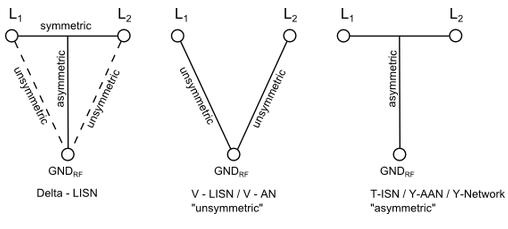
\includegraphics[scale=0.65]{f1.png}
\end{figure}\\
\indent Odbiornik testowy może posiadać detektory: wartości szczytowej - PeaK pokazujący wartość maksymalną w czasie, wartości średniej - AVerage pokazujący wartość średnią, lecz nie mówiący nic o amplitudach oraz wartości quasi - szczytowej, czyli Quasi Peak odzwierciedlający amplitudę, a~także współczynnik wypełnienia.
\section{Cel ćwiczenia}
\indent\indent Celem wykonywanego ćwiczenia jest przeprowadzenie pomiarów przewodzonych zaburzeń radioelektrycznych oraz zdefiniowanie zgodności badanego urządzenia z odpowiednimi normami. Pozwoli to na zapoznanie się z~aparaturą pomiarową - odbiornikiem testowym, a także działaniem sieci sztucznej (LISN). Dla poprawnego wykonania ćwiczenia konieczne jest także zapoznanie się z odpowiednimi normami. Do planowanych badań emisyjności zaburzeń przez zasilacz do laptopa, należy odnieść się do normy PN-EN 55022 dotyczącej urządzeń informatycznych.
\section{Spis wykorzystanych urządzeń}
\begin{itemize}
\item Odbiornik testowy Rhode \& Schwarz ESL-3,
\item Sieć sztuczna EMCO MODEL 3810/2 LISN,
\item EUT (Equipment Under Test) - urządzenia testowane:
\begin{itemize}
\item Ładowarka do laptopa Lenovo, model ADLX65NCC3A,
\item Zasilacz dostępny w laboratorium na stanowisku pomiarowym.
\end{itemize}
\end{itemize}
\begin{figure}[h!]
\centering
\caption{Specyfikacja wykorzystanej sieci sztucznej}
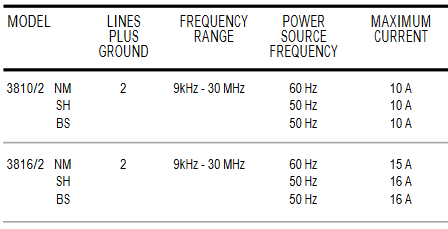
\includegraphics[scale=0.5]{f2.png}
\end{figure}
\begin{figure}[h!]
\centering
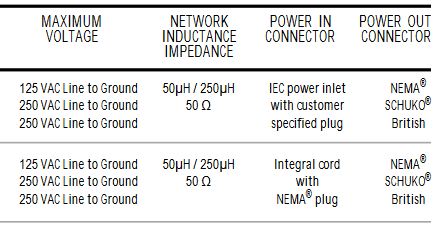
\includegraphics[scale=0.5]{f3.png}
\end{figure}
\section{Przebieg ćwiczenia}
\indent\indent Podczas wykonywania ćwiczenia można wydzielić trzy główne etapy:
\begin{enumerate}
\item przygotowanie do ćwiczenia,
\item uruchomienie i konfiguracja aparatury pomiarowej,
\item wykonanie pomiarów.
\end{enumerate}
\indent\indent Po ukończeniu pierwszego etapu - zapoznaniu się z instrukcją stanowiskową, zanotowaniu modeli sprzętu wykorzystywanego do badań oraz uzyskaniu zgody prowadzącego rozpoczęto konfigurację aparatury pomiarowej.\\
\indent Drugi etap polegał na konfiguracji odbiornika testowego zgodnie z instrukcją. Wykonano kolejno: konfigurację wstępną, ustawienie urządzenia pomiarowego w tryb pracy odbiornika pomiarowego, włączenie TRACE 1 i 2 oraz skonfigurowanie kolejno detektorów QP i AVG, dodanie poziomów normatywnych - wybrano normę PN-EN 55022 dla urządzeń informatycznych, wprowadzenie domyślnej konfiguracji pomiaru zautomatyzowanego. Należało także przygotować stanowisko pomiarowe zgodnie z przedstawionym w~instrukcji wyciągiem z norm oraz podłączyć wszystkie urządzenia, aby można było przeprowadzić pomiary.\\
\indent Po akceptacji konfiguracji odbiornika testowego przez prowadzącego rozpoczęto pomiary. Dla zasilacza Lenovo przeprowadzono sześć pomiarów - po trzy poziomy obciążenia dla linii L1 - fazowa oraz L2 - neutralna. Pierwszy poziom obciążenia to zasilacz niepodłączony do odbiornika. Drugi poziom to zasilacz podłączony do odbiornika pracującego na niskim obciążeniu. Na trzecim poziomie odbiornik został poddany wysokiemu obciążeniu na czas trwania pomiaru.\\
Dla zasilacza dostępnego na stanowisku przeprowadzony został wyłącznie jeden pomiar - na linii L1, przy konfiguracji 1 - brak podłączonego odbiornika. Dla tego urządzenia przekroczone zostały w~sposób znaczny normy dotyczące zarówno pomiarów detektorem QP, jak i detektorem AV. Dalsze pomiary byłyby pozbawione sensu, ponieważ urządzenie nie spełniło norm podczas jednego z~planowanych badań i~ewentualna zgodność z~normami w dalszych badaniach i~tak nie pozwoliłoby na dopuszczenie urządzenia na rynek.
\clearpage
\section{Wyniki pomiarów}
\subsection{Linia 1}
\begin{figure}[h!]
\centering
\caption{Wyniki pomiarów dla zasilacza Lenovo - linia 1, brak obciążenia}
\includegraphics[scale=0.34]{Linia1/k1.png}
\end{figure}\bigskip
\begin{figure}[h!]
\centering
\caption{Wyniki pomiarów dla zasilacza Lenovo - linia 1, lekkie obciążenie}
\includegraphics[scale=0.34]{Linia1/k2.png}
\end{figure}
\clearpage
\begin{figure}[t]
\centering
\caption{Wyniki pomiarów dla zasilacza Lenovo - linia 1, mocne obciążenie}
\includegraphics[scale=0.34]{Linia1/k3.png}
\end{figure}
\begin{figure}[b]
\centering
\caption{Wyniki pomiarów dla zasilacza dostępnego na stanowisku - linia 1, brak obciążenia}
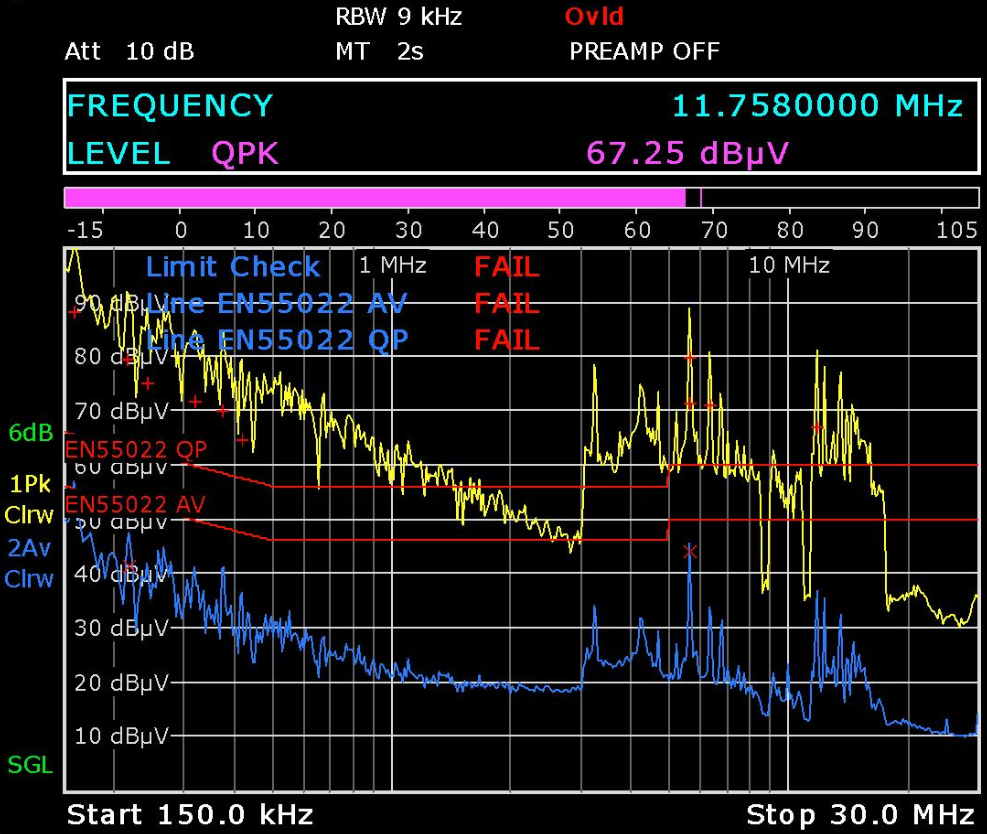
\includegraphics[scale=0.34]{Linia1/stary_k1.png}
\end{figure}
\clearpage
Na rys. 3 - 5 przedstawione są wartości zaburzeń przewodzonych emitowanych przez zasilacz Lenovo dla różnych poziomów obciążenia. Każdy z wykresów posiada naniesione wartość graniczne dla detektorów QP oraz AV zgodnie z normą EN55022. Otrzymane na wykresie wartości oddalone są od krzywej granicznej o 10 - 20 dB, co wymagałoby wzrostu napięcia 10 - 100 razy, aby przekroczyć normy. Pomiar jest więc z całą pewnością wiarygodny, a~badany zasilacz spełnia wymagania stawiane przez normę EN55022. Peak List dla zasilacza nie zawiera żadnych elementów, ponieważ zarówno detektor wartości szczytowej, jak i detektor wartości średniej nie wykryły zaburzenia zbliżającego się na odległość mniejszą niż 6 dB od wartości wynikających z wyżej wymienionej normy. Przy braku obciążenia zaburzenia obserwowane są dla częstotliwości mniejszych niż 1~MHz. Dla lekkiego obciążenia obserwuje się niewielkie zaburzenia wąskopasmowe dla częstotliwości 500 - 600 kHz oraz dla częstotliwości powyżej 10 MHz. Przy dużym obciążeniu jednym obszarem wolnym od zaburzeń jest przedział częstotliwości 1 - 2 MHz.\\
\indent Zasilacz dostępny na stanowisku laboratoryjnym w wielu punktach znacząco przekracza dopuszczalne poziomy emitowanych zaburzeń dla detektora PK (rys. 6). Dla wartości bliskich dopuszczalnych przez normę oraz dla większych niż dopuszczalne wykonywany jest automatyczny domiar detektorem QP. Pozwala on na uzyskanie większej dokładności. Parametry oraz wyniki domiaru zostały zebrane w tab. 1. Ze względu na duże wahania amplitudy zaburzeń, wartość średnia podczas całego badania znajduje się w normie, co świadczy o jej niedokładności jako metodzie pomiaru.
\subsection{Linia 2}
\begin{figure}[h!]
\centering
\caption{Wyniki pomiarów dla zasilacza Lenovo - linia 2, brak obciążenia}
\includegraphics[scale=0.34]{Linia2/k1.png}
\end{figure}
\clearpage
\begin{figure}[t!]
\centering
\caption{Wyniki pomiarów dla zasilacza Lenovo - linia 2, lekkie obciążenie}
\includegraphics[scale=0.34]{Linia2/k2.png}
\end{figure}
\begin{figure}[h!]
\centering
\caption{Wyniki pomiarów dla zasilacza Lenovo - linia 2, mocne obciążenie}
\includegraphics[scale=0.34]{Linia2/k3.png}
\end{figure}
Z rys. 7 - 9 dla badań zasilacza Lenovo dla linii L2 wynika, że występuje mniej zaburzeń przy braku obciążenia. Są one widoczne jedynie dla częstotliwości 170 - 200 kHz. Przy lekkim obciążeniu zaburzenia można obserwować dla częstotliwości 500 - 600 kHz, a także większych niż 10 MHz. przy dużym obciążeniu wyraźne zaburzenia powstają w paśmie zbliżonym do obciążenia lekkiego.
\clearpage
\subsection{Peak List}
\begin{table}[h!]
  \centering
  \caption{Peak List dla pomiaru zasilacza będącego wyposażeniem stanowiska pomiarowego}
    \begin{tabular}{|c|c|c|c|}\hline
    \multicolumn{2}{|c|}{Type} & \multicolumn{2}{|c|}{ESL-3} \\\hline
    \multicolumn{2}{|c|}{Version} & \multicolumn{2}{|c|}{1.83 SP1} \\\hline
    \multicolumn{2}{|c|}{Date} & \multicolumn{2}{|c|}{13.Nov 17} \\\hline
    \multicolumn{2}{|c|}{Mode} & \multicolumn{2}{|c|}{Receiver} \\\hline
    \multicolumn{2}{|c|}{Start} & \multicolumn{2}{|c|}{150 kHz} \\\hline
    \multicolumn{2}{|c|}{Stop} & \multicolumn{2}{|c|}{30 GHz} \\\hline
    \multicolumn{2}{|c|}{x-Axis} & \multicolumn{2}{|c|}{LOG} \\\hline
    \multicolumn{2}{|c|}{Scan Count} & \multicolumn{2}{|c|}{1} \\\hline
    \multicolumn{4}{|c|}{Scan 1:} \\\hline
    \multicolumn{2}{|c|}{Start} & \multicolumn{2}{|c|}{150 kHz} \\\hline
    \multicolumn{2}{|c|}{Stop} & \multicolumn{2}{|c|}{30 GHz} \\\hline
    \multicolumn{2}{|c|}{Step} & \multicolumn{2}{|c|}{4 kHz} \\\hline
    \multicolumn{2}{|c|}{RBW} & \multicolumn{2}{|c|}{9 kHz} \\\hline
    \multicolumn{2}{|c|}{Meas Time} & \multicolumn{2}{|c|}{0.05 s} \\\hline
    \multicolumn{2}{|c|}{Auto Ranging} & \multicolumn{2}{|c|}{OFF} \\\hline
    \multicolumn{2}{|c|}{RF Att} & \multicolumn{2}{|c|}{10 dB} \\\hline
    \multicolumn{2}{|c|}{Auto Preamp} & \multicolumn{2}{|c|}{OFF} \\\hline
    \multicolumn{2}{|c|}{Preamp} & \multicolumn{2}{|c|}{0 dB} \\\hline
    \multicolumn{4}{|c|}{TRACE 1 FINAL:} \\\hline
    \multicolumn{2}{|c|}{Trace Mode} & \multicolumn{2}{|c|}{CLR/WRITE} \\\hline
    \multicolumn{2}{|c|}{Final Detector} & \multicolumn{2}{|c|}{QUASI PEAK} \\\hline
    \multicolumn{2}{|c|}{x-Unit} & \multicolumn{2}{|c|}{Hz} \\\hline
    \multicolumn{2}{|c|}{y-Unit} & \multicolumn{2}{|c|}{dB$\mu$V} \\\hline
    \multicolumn{2}{|c|}{Final Meas Time} & \multicolumn{2}{|c|}{2 s} \\\hline
    \multicolumn{2}{|c|}{Margin} & \multicolumn{2}{|c|}{6 dB} \\\hline
    \multicolumn{2}{|c|}{Values} & \multicolumn{2}{|c|}{13} \\\hline
    Trace & Frequency [kHz] & Level [dB$\mu$V] & $\Delta$ Limit [dB] \\\hline
    1 & 158   & 88.14 & 22.57157 \\\hline
    2 & 158   & 51.48 & -4.08843 \\\hline
    1 & 214   & 79.44 & 16.3914 \\\hline
    2 & 218   & 41.54 & -11.3548 \\\hline
    1 & 242   & 75.25 & 13.2227 \\\hline
    1 & 318   & 71.75 & 11.99114 \\\hline
    1 & 374   & 69.98 & 11.56838 \\\hline
    1 & 418   & 64.55 & 7.062203 \\\hline
    1 & 5 618   & 71.24 & 11.24 \\\hline
    1 & 5 634   & 79.72 & 19.72 \\\hline
    2 & 5 634   & 44.1 & -5.9 \\\hline
    1 & 6 342   & 70.89 & 10.89 \\\hline
    1 & 11 758   & 67.01 & 7.01 \\\hline
    \end{tabular}%
  \label{tab:addlabel}%
\end{table}%
W tab. 1 zostały zebrane dane o parametrach pomiaru oraz punktach, w których normy zostały przekroczone lub wyniki były bliskie przekroczenia norm. Dla tych punktów został wykonany domiar detektorem QP. To pozwoliło ustalić dokładniejszą wartość emitowanych zaburzeń dla danej częstotliwości. Wartość $\Delta$ Limit pokazuje o ile dB przekroczona została norma dla danej częstotliwości. Jeśli jest ujemna, to oznacza, że wartość pomiaru znalazła się poniżej normy. Jak można zauważyć, detektor AV, pomimo zbliżania się do maksymalnej wartości dopuszczanej w~normie, nie przekroczył jej. Największe przekroczenie normy - o 22.57 dB - odnotowano detektorem QP dla częstotliwości 158 kHz.
\section{Wnioski}
\begin{itemize}
\item Dla badań przeprowadzonych na linii L1, na trzech poziomach obciążenia zasilacza do laptopa Lenovo została potwierdzona jego zgodność z normą EN55022 dla detektorów AV oraz QP.
\item Podobne wyniki otrzymywane są podczas badań linii L2, jednak tam zaburzenia mają mniejsze wahania i występują dla węższych pasm.
\item Zasilacz dostępny w laboratorium w sposób znaczny przekroczył dopuszczalne normy. Zostały przeprowadzone badania wyłącznie bez obciążenia dla linii L1, ponieważ przy niespełnieniu normy chociaż raz należy go uznać za niezdatny do użytku. Przeprowadzanie dalszych pomiarów byłoby bezcelowe pod kątem badania zgodności z normami.
\item Po odnotowaniu wartości bliskich lub wyższych od normy podczas pomiaru wstępnego dla detektora PK, wykonany został automatycznie pomiar końcowy detektorem QP. Normy definiowane są dla detektorów AVG oraz QP, jednak pomiar wstępny wykonuje się z wykorzystaniem PK oraz AVG, ponieważ użycie QP, który w~pewien sposób pokazuje sygnał ważony, byłoby zbyt czasochłonne. Zestawienie częstotliwości, dla których wykonany został domiar przedstawiono w tab. 1.
\end{itemize}
\clearpage
\section{Literatura}
[1] J. Bogucki, A. Chudziński, J. Połujan, ,,Emisja elektromagnetyczna urządzeń w praktyce'',\\ Instytut~Łączności - Państwowy Instytut Badawczy\newline\newline
[2] Dane katalogowe firmy Rhode \& Schwarz\newline\newline
[3] http://www.schwarzbeck.de/en/lisn-line-impedance-stabilisation-networks.html \newline\newline
\end{document}